\documentclass{jfm}

%PACKAGES
\usepackage{graphicx}
\usepackage{color}
\usepackage[dvipsnames]{xcolor}
\usepackage{amsmath}
\usepackage{amssymb}
\usepackage{siunitx} % Nice units
\usepackage{hyperref}
\usepackage{pgfplots}
    %\pgfplotsset{compat=1.13}
% \usepackage[ margin = 1in]{geometry}
\usepackage{wasysym}
\usepackage[titletoc,toc,title]{appendix}
\usepackage{setspace}
\usepackage{natbib}
\usepackage{bm}
\usepackage{float}
\usepackage{subfigure}
\usepackage{cancel}
\usepackage[normalem]{ulem}

%% New commands
\newcommand{\MM}[1]{[\textcolor{blue}{#1 }]}
\newcommand{\DA}[1]{[\textcolor{ForestGreen}{#1 }]}
\newcommand{\eps}{\varepsilon}
\newcommand{\ifl}{^{(i)}}
\newcommand{\efl}{^{(e)}}
\newcommand{\iande}{^{(i,e)}}


\title{Controlling Wavebreaking in Dispersive Hydrodynamic Media}
\author{D.A. Anderson}
\author{M.D. Maiden}
\author{M.A. Hoefer}
\affiliation{Department of Applied Mathematics, University of Colorado, Boulder, Colorado 80309, USA}
\date{\today}
\begin{document}

% \newtheorem{lemma}{Lemma}
% \newtheorem{corollary}{Corollary}

\author
 {
 Dalton V. Anderson\aff{1}\aff{2}
  \corresp{\email{dalton.anderson@colorado.edu}},
  Mark A. Hoefer \aff{1}
  \and 
  Michelle D. Maiden\aff{1}
  }

\affiliation
{
\aff{1}
Department of Applied Mathematics, University of Colorado, Boulder, CO 80302, USA
\aff{2}
Department of Aerospace Engineering, University of Colorado, Boulder, CO 80302, USA
}

\maketitle

\begin{abstract}
Dispersive hydrodynamic systems exhibit a rich variety of behavior, depending on the initial value problem considered. However, many such systems can only be experimentally controlled at one boundary. Here, a method is presented for generating an initial condition via a boundary value problem formulation for nonlinear dispersive partial differential equations, which model such systems. The conduit equation is chosen due to its high fidelity to physical experiments. The dispersionless limit of the conduit equation is taken and evolved backwards in time from the desired initial condition of a step increase of a constant background at a chosen point in space and time. This method is tested for various step sizes and positions of the step. Experiments on this method agree well with theory, having an upper bound of 10\%, which is consisten with other conduit experiments.
\end{abstract}

\section{Introduction}\label{sec:Intro}
Dispersive shock waves (DSWs) are coherent structures that exhibit the interplay of nonlinearity and dispersion. A DSW is an expanding, oscillating train of amplitude-ordered nonlinear waves composed of a large amplitude solitary wave adjacent to a monotonically decreasing wave envelope that terminates with a packet of small amplitude dispersive waves. These structures are pervasive in dispersive hydrodynamic systems, having been observed in 
quantum systems (ultra-cold atoms \cite{dutton_observation_2001,hoefer_dispersive_2006}, semiconductor cavities \cite{amo_polariton_2011}, 
electron beams \cite{mo_experimental_2013}), 
nonlinear optics \cite{rothenberg_observation_1989},
geophysical fluids \cite{hammack_korteweg-vries_1978,farmer_generation_1999}, and
rarefied plasma \cite{taylor_observation_1970}. %,tran_shocklike_1977}.
However, experimental generation and analysis of DSWs remains a difficult and expensive problem in many of these systems, constrained by expensive laboratory setups
\cite{dutton_observation_2001,hoefer_dispersive_2006,mo_experimental_2013,hammack_korteweg-vries_1978}
challenging field studies \cite{farmer_generation_1999},
difficulties in capturing dynamical information \cite{rothenberg_observation_1991,dutton_observation_2001,hoefer_dispersive_2006},
complex physical modeling \cite{farmer_generation_1999}, or a loss of
coherence due to multi-dimensional instabilities \cite{dutton_observation_2001,amo_polariton_2011} or dissipation \cite{taylor_observation_1970,mo_experimental_2013}.  

Many of these difficulties have been overcome by utilizing a model dispersive hydrodynamics system: the conduit system. 
This system enables high fidelity studies of large amplitude DSWs,
which are found to agree quantitatively with nonlinear wave averaging
or Whitham theory
\cite{whitham_linear_1974,gurevich_nonstationary_1974,lowman_dispersive_2013,maiden_observation_2016}. 
However, the conduit system can only be controlled at one boundary, which makes the initial condition DSW problem difficult to study.
Here, we report on a mathematical tool that is a feasible way to achieve wavebreaking away from boundary effects. 
We take the dispersionless limit of the conduit equation and evolve the step initial condition backwards in time.
The resulting solution can be used as a boundary condition for the conduit equation and evolved forwards in time to yield the desired step in the full conduit system.

The following paper is organized as follows. Section \ref{sec:Theory} is the theoretical section and includes background information on the conduit equation and the mathematical procedure for converting the initial value problem to a boundary value problem. Section \ref{sec:Exp} is the experimental section and covers both numerical and experimental methods and analysis. Section \ref{sec:Dis} is a discussion of the major results of the previous two sections, and conclusions are in Section \ref{sec:Con}.

\section{Theory}\label{sec:Theory}
\subsection{Conduit Equation}
Conduits generated by the low Reynolds number, buoyant dynamics of two miscible fluids with differing densities and viscosities were first studied in the context of geological and geophysical processes \cite{whitehead_dynamics_1975}. 
Here, we focus on viscous fluid conduits, which can be realized physically with a sugar solution or using glycerin for the exterior fluid, and a dyed, diluted version of the same fluid as the interior fluid \cite{olson_solitary_1986,scott_observations_1986,whitehead_wave_1988,maiden_observation_2016}.
Perturbations around a constant background conduit with the assumptions of long-wavelength, slow-time, and slow-space result in the conduit equation, a (1+1)-D dispersive hydrodynamic equation with a nonlinear, nonlocal dispersive term \cite{lowman_dispersive_2013}.
This paper focuses on the realization of the Gurevich-Pitaevskii (GP) problem \cite{gurevich_nonstationary_1974}, a standard textbook problem for the study of DSWs \cite{el_dispersive_2016}, for the conduit equation
\begin{equation}\label{eq:conduit}
  A_t + (A^2)_z -(A^2(A^{-1}A_t)_z)_z = 0.
\end{equation}

\noindent
This equation approximately governs the evolution of the circular
interface with cross-sectional area $A$, in vertical space $z$ and time $t$. This interface separates a light, viscous
fluid rising buoyantly through a heavy, more viscous fluid
at small Reynolds numbers in the long-wavelength, slow-time regime \cite{scott_observations_1986,lowman_dispersive_2013}.
Here, the GP problem is the study of the dispersive hydrodynamics of an initial step increase in conduit area 
\begin{equation}\label{eq:GP}
    A(z,t) = \begin{cases}
                A_1, & z\geq z_b \\
                A_2, & z<z_b
             \end{cases},
\end{equation}
for some $A_2>A_1$. 
Note that since the conduit equation obeys the scaling invariance
\begin{equation}\label{eq:scaling1}
  \begin{array}{ccc}
    \tilde{A}=A/A_0, & \tilde{z}=A_0^{-1/2}z,  & \tilde{t} = A_0^{1/2}t,
  \end{array}
\end{equation}
this is equivalent to studying
\begin{equation}\label{eq:GPscaled}
    A(z,t) = \begin{cases}
                1,   & z\geq z_b \\
                A_b, & z<z_b
             \end{cases},
\end{equation}
where $A_b = A_2/A_1 > 1$.

\subsection{Inviscid Burgers Equation}\label{sec:Inv-Bur-EQ}

% \begin{itemize}
% 	\item Assume dispersion is small prior to breaking
% 	\item Rarefaction Wave Solution
% 	\item Inviscid Burgers: $A_t + 2AA_z = 0$.
% \end{itemize}

To implement our method, we assume prior to DSW breaking, dispersive behavior is minimal. 
Intuitively, this assumption is valid because the GP problem connects two constant states, so no oscillitory behavior is observed.
Therefore, we can safely neglect the dispersive term, $(A^2(A^{-1}A_t)_z)_z$, and focus on the inviscid Burgers Equation
\begin{equation}\label{eq:IBE}
	u_\tau + \left(u^2\right)_\zeta = 0  
\end{equation}
Here, we consider two main solution families of Eq.~\ref{eq:IBE}: constants and the self-similar solution $u(\zeta,\tau) =  \frac{\zeta}{2\tau}$, called the rarefaction wave solution. 
This solution family is unbounded in $u$, thus in order to make the problem physical, we define a piecewise solution that connects two constant states $u_-<u_+$ with the rarefaction wave solution
\begin{equation}\label{eq:raresoln}
   u(\zeta,\tau) = \begin{cases}
               u_- & : \zeta\le \zeta_-\\
               \frac{\zeta}{2\tau} & : \zeta_- \le \zeta \le \zeta_+\\
               u_+ & :\zeta\ge \zeta_+
            \end{cases},
\end{equation}  
where $\zeta_\pm$ denote the connection of the rarefaction wave solution to $u_\pm$, respectively. %An example of this is shown in Fig. \ref{fig:rare_wave}.


 Note $\zeta_+$ and $\zeta_-$ bifurcate from the origin at speeds $c_+$ and $c_-$, where continuity conditions require
\begin{equation}
   \lim_{\zeta_\to \zeta_\pm} \frac{\zeta}{2\tau} = u_\pm 
   \Rightarrow  c_\pm \tau/2\tau=u_\pm 
   \Rightarrow c_\pm=2u_\pm
\end{equation}
Therefore, $\zeta_\pm(\tau) = 2u_\pm t$.

Although Eq. \ref{eq:raresoln} is not differentiable everywhere, it is a weak solution, i.e. a solution of the integral form of Eq.~\ref{eq:IBE}
    \begin{equation}
       \frac{d}{d\tau} \int_a^b u(\zeta,\tau)d\zeta = -u^2\Big|_{\zeta=a}^b.
    \end{equation}
Now, it remains to convert this solution into the physical coordinate system. 
Using the expressions found for $\zeta_\pm$
\begin{equation}
   u(\zeta,\tau) = \begin{cases}
               u_- & : \zeta\le 2u_-\tau  \\
               \frac{\zeta}{2\tau} & : 2u_-\tau \le \zeta \le 2u_+\tau\\
               u_+ & :\zeta\ge 2u_+\tau
            \end{cases},
\end{equation}
we will now make the necessary substitutions. Note the desired solution breaks for a generic $(z_b,t_b)$, $ 1 \le A_b$, and $A(0,0) = 1$, and further making the simplifying assumption of an initial conduit with unit area
\begin{equation} \label{eq:coordSub1}
\begin{array}{ccc}
    \zeta = -(z-z_b), & \tau = -(t-t_b) ,& t_b = \frac{z_b}{2}\\
    u_- = 1 , &                    &u_+ = A_b 
\end{array}
\end{equation}
Then the requisite boundary condition for Eq.~\ref{eq:conduit} has the form
\begin{equation}\label{eq:BCDSW}
   A(0,t) = 
     \begin{cases}
       1                    & :                        t \le 0                          \\
       \frac{1}{1-2t/z_b}  & :  0 < t/z_b < \frac{(A_b - 1)}{2A_b}          \\
       A_b                  & :        t/z_b \ge  \frac{(A_b - 1)}{2A_b}
     \end{cases}.
\end{equation}
An example of this solution and its evolution is shown in Fig. \ref{fig:rare_wave_inv}. \MM{This figure doesn't exactly match up, as in the figure, the solution is shown for specific $t$-values for all $z$, whereas this equation is for all $t$ with $z=0$. Maybe add a subfigure showing the boundary condition?}


\begin{figure}
    \centering
       \subfigure[Profile in $t$]{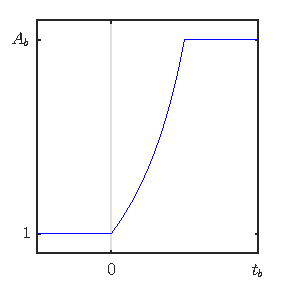
\includegraphics{Figures/BC_wave.pdf}}
	\subfigure[Profile in $z$]{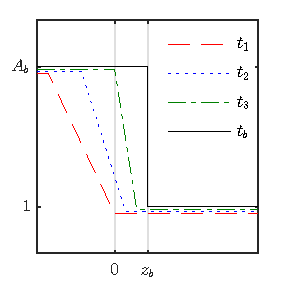
\includegraphics[height = 2in]{Figures/inv_rw}}     
    \caption{(a) Dimensional version of the boundary condition Eq.~\ref{eq:BCDSW}. (b) Evolution of the rescaled piecewise rarefaction wave Eq.~\ref{eq:BCDSW}. Note as time moves forward, the wave approaches the desired step.}
    \label{fig:rare_wave_inv}
\end{figure}


\subsubsection{Dimensionalization}\label{sec:Dimensionalization}
Next, we rescale Eq.~\ref{eq:BCDSW} from the nondimensional conduit equation (tilded variables) to physical parameters (plain variables). 
Following the scaling given in \cite{lowman_dispersive_2013}, denote by $f^{(i,e)}$ as the fluid property $f$ for the interior or exterior fluid, $\mu$ as a fluid's dynamic viscosity, and $\rho$ as its density. Then defining $R_0$ as the (dimensional) conduit radius, and $Q_0$ as the (dimensional) flow rate, we have
\begin{equation}
\begin{split}
    \begin{array}{ccc}
        \Delta = \rho\efl-\rho\ifl       & \eps = \frac{\mu\ifl}{\mu\efl}, & \alpha = \left(\frac{2^7\mu\ifl}{\pi g \Delta}\right)^{1/4} \\
        \tilde{R} = R/L, & \tilde{z} = \eps^{1/2}z/L,       & L = R_0/\sqrt{8} \\
    \multicolumn{3}{c}
    { 
        \begin{array}{cc}
            \tilde{t} = \eps^{1/2}t/T,                 & T = \frac{\sqrt{8}\mu\ifl}{g R_0 \Delta} \\
            \tilde{u} = u/U,                 & U = \frac{g R_0^2 \Delta}{8 \mu\ifl} \\
            \tilde{A} = A/A_0,               & A_0 = \frac{\alpha^2 Q_0^{1/2}}{32} \\
        \end{array}
    }
    \end{array}
    \end{split}
\end{equation}
Then rescaling \ref{eq:BCDSW} results in a volumetric flow rate profile with an area ratio of $A_b$ and a predicted break height of $z_b$
\begin{equation}\label{eq:FlowRateProfile}
   Q(t) = Q_0
     \begin{cases}
       1                    & :                        t \le 0                          \\
       \frac{1}{(1-2\frac{U}{z_b}t)^2}  & :  0 < \frac{U}{z_b}t < \frac{(A_b - 1)}{2A_b}          \\
       A_b^2                  & :        \frac{U}{z_b}t \ge  \frac{(A_b - 1)}{2A_b}
     \end{cases}.
\end{equation}

\subsection{Generalization of Technique}\label{sec:Gen-Tech}
\MM{Move to end of \ref{sec:Inv-Bur-EQ}?}
This method of neglecting the dispersive term can be used to generate a variety of initial conditions. In Figs.~\ref{fig:chars1} \& \ref{fig:chars2}, we show characteristic plots based on the dispersionless approach to generate a DSW in Fig.~\ref{fig:chars1}, a box in Fig.~\ref{fig:chars2}(a), a triangle in Fig.~\ref{fig:chars2}(b), and an N-wave in Fig.~\ref{fig:chars2}(c).


\begin{figure}
  \centering
  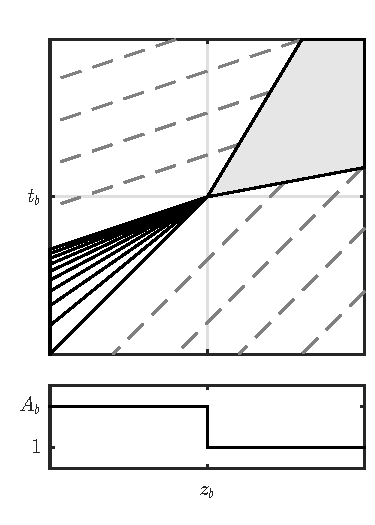
\includegraphics{Figures/char_dsw.pdf}
  \caption{}
  \label{fig:chars1}
\end{figure}



\begin{figure}
  \centering
  \subfigure[box]{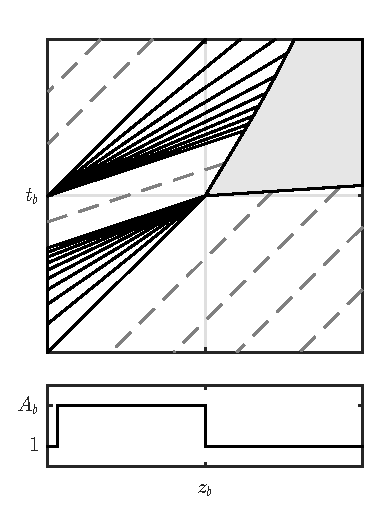
\includegraphics{Figures/char_box.pdf}}
  \subfigure[triangle]{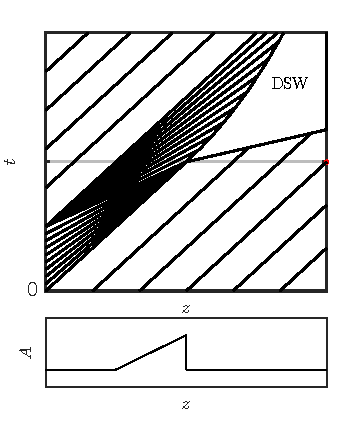
\includegraphics{Figures/char_triangle.pdf}}
  \subfigure[N]{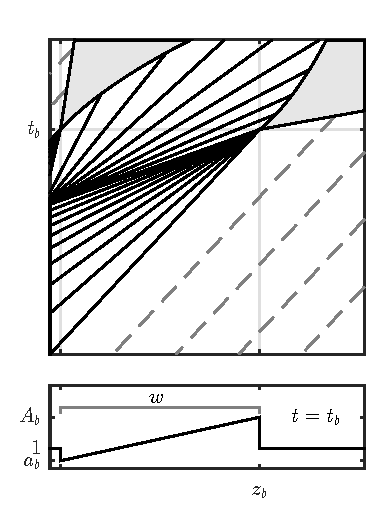
\includegraphics{Figures/char_N.pdf}}
  \caption{}
  \label{fig:chars2}
\end{figure}

\section{Experiment}\label{sec:Exp}
	\begin{itemize}
	    \item \textbf{Setup:} Apparatus, Camera, Pump
	    \item \textbf{Methods: }Image Processing
	    \item Determining Wavebreaking
	    \item Uncertainty Quantification 
	\end{itemize}
	\subsection{Setup}
	
The experimental apparatus shown in Fig. \ref{fig:expsys}(a) consists of a square acrylic column with dimensions  $\SI{4}{\centi\meter} \times \SI{4}{\centi\meter} \times \SI{92}{\centi\meter}$; the column is filled with a highly viscous, transparent, exterior fluid - either corn syrup or glycerin. 
A nozzle is installed at the base of the column to allow for the injection of the interior fluid. To eliminate surface tension effects, the interior fluid is a solution of the exterior fluid (glycerin or corn syrup), deionized water, and black food coloring. 
Resultantly, the interior fluid has both lower density and viscosity than the exterior fluid $(\mu^{(i)} \ll \mu^{(e)}$ , $\rho^{(i)} < \rho^{(e)})$.

Interior fluid is drawn from a separate reservoir and injected through the nozzle via a high precision piston pump controlled by a computer. 
The interior fluid rises buoyantly due to the density difference between interior and exterior fluids. By injecting at a constant rate, a vertically uniform fluid conduit is established. This ``fluid conduit" is referred to as the background conduit. 
Data acquisition is done using a high resolution camera equipped with a macro lens at the predicted break height.\MM{Should we include brand names???} 
A ruler is positioned beside the column to determine the observed break height. 



\begin{figure}
\centering
\subfigure[]{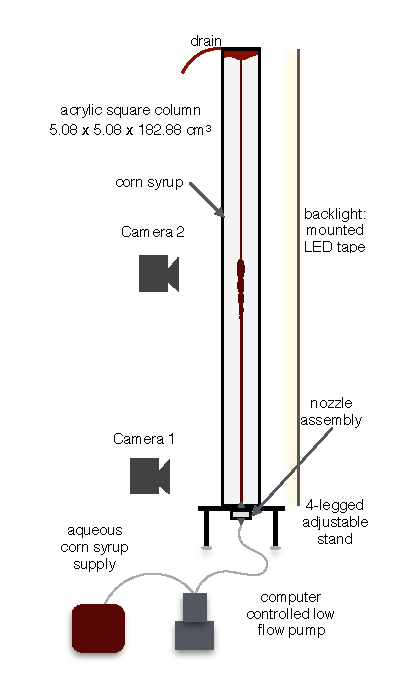
\includegraphics[height = 3in]{Figures/expt_setup}}
\subfigure[]{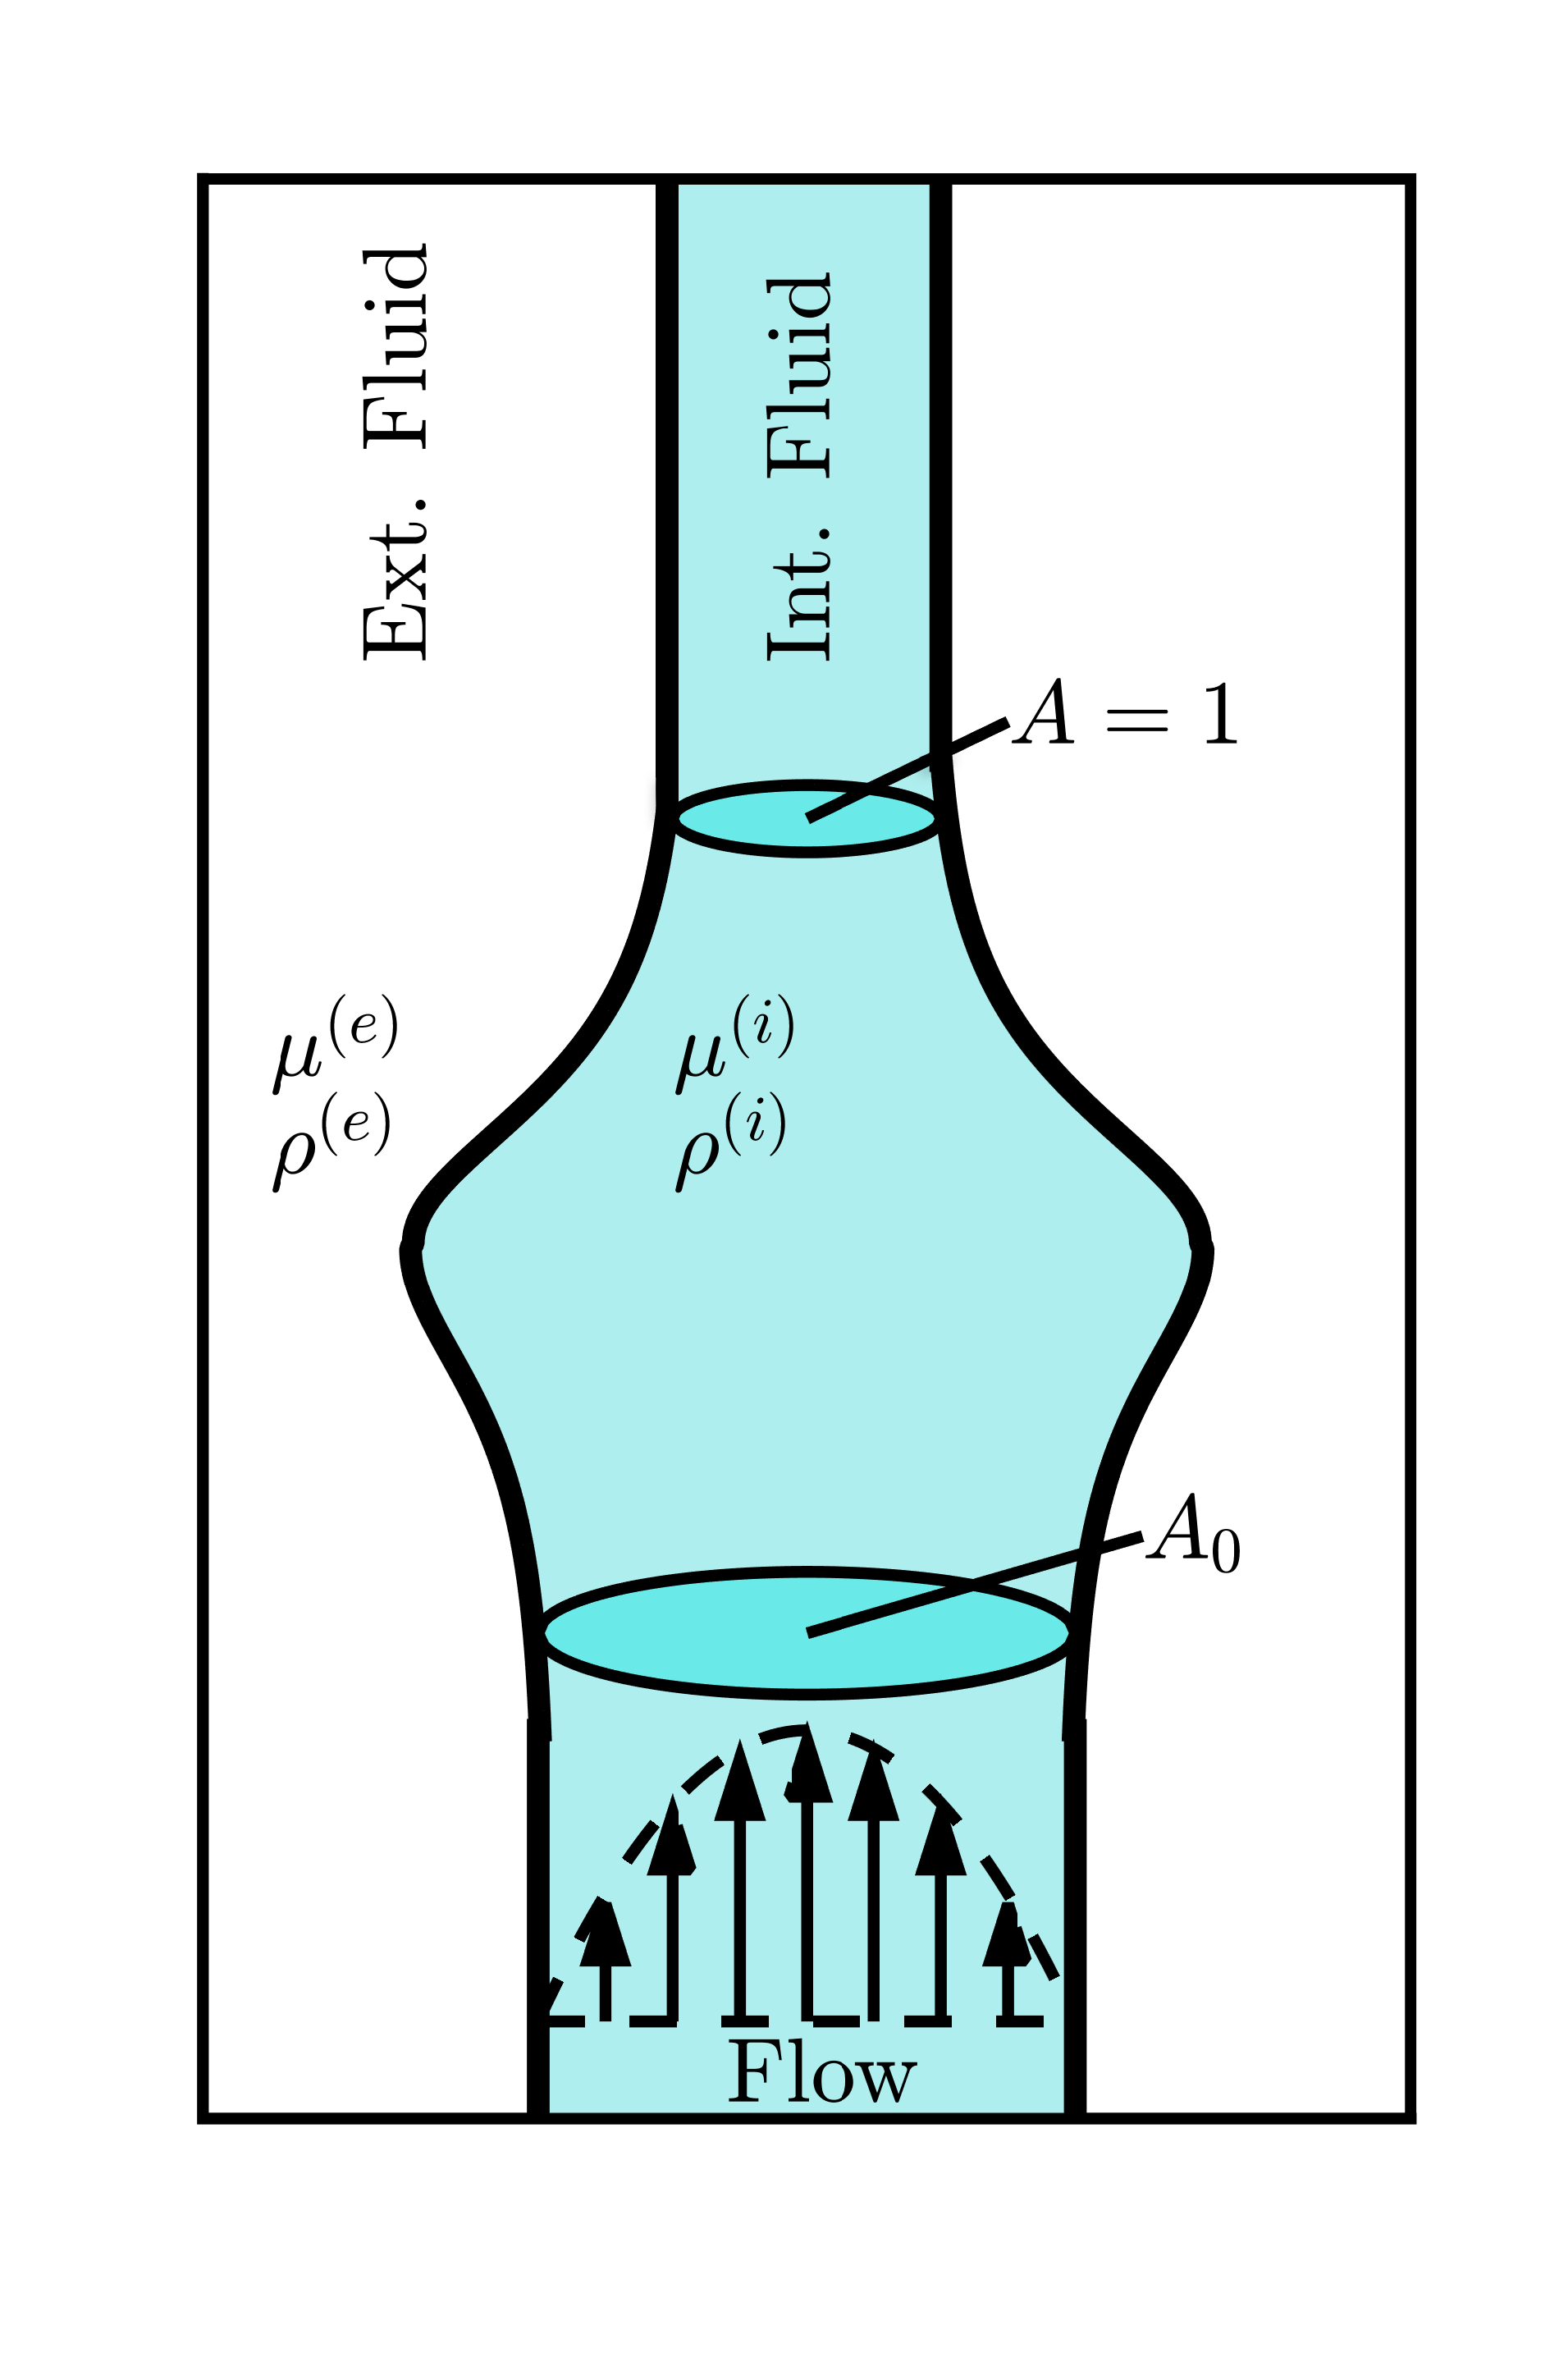
\includegraphics[height = 3in]{Figures/conduit.png}}
\caption{(a) Schematic of the experimental setup. \MM{Add ruler? Add computer connected to pump?} (b) Schematic of the conduit near $t=t_b$. Note that dispersion causes the step to ``smooth out".}
\label{fig:expsys}
\end{figure}

\begin{figure}
\centering
\subfigure[]{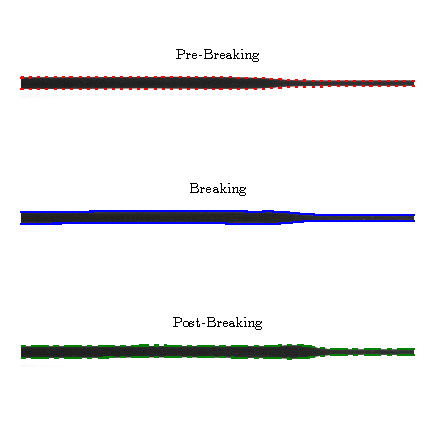
\includegraphics[height = 2.5in]{Figures/BreakEdgeDetection.pdf}}
\subfigure[]{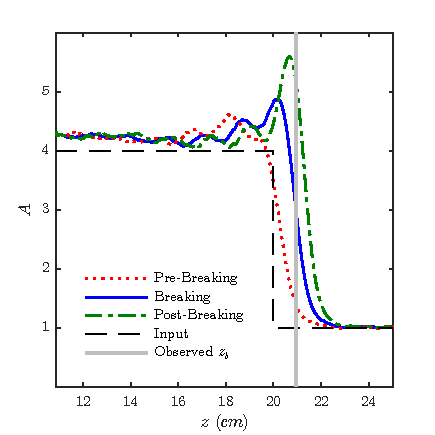
\includegraphics[height = 2.5in]{Figures/BreakEdges.pdf}}
\caption{(a) Processed images from a glycerin trial with $\mu\ifl = 72\pm1 \si{cP}$, $\rho\ifl = 1.222\pm0.001 \si{g/cm^3}$, $\mu\efl = 1190\pm 20 \si{cP}$, $\rho\efl = 1.262\pm0.001\si{g/cm^3}$, and $Q_0 = 0.25\pm 0.01 \si{ml/min}$. The grayscale images are overlayed with the extracted conduit edges and the conduit centerline. (b) Area plot corresponding to the images in (a). The dashed line\MM{s} indicate the threshold\MM{s} for the global maximum \MM{and local minimum}. \MM{Add a line that shows the breaking height. Check to make sure vertical distance is correct.}}
\label{fig:BreakEdge}
\end{figure}

    
	\subsection{Methods}
	For each trial, a volumetric flow rate profile $Q(t)$ is generated using Eq.~\ref{eq:FlowRateProfile} for the chosen $z_b$ and $A_b$. 
	The predicted time of breaking, $t_b$, is $t_b=z_b/2U$.
	The camera takes several high-resolution images before, during, and after the time of breaking.
	A schematic of the conduit near the height and time of breaking is shown in Fig. \ref{fig:expsys}(b).
	After breaking occurs, the pump is reduced to the background rate $Q_0$, and the conduit is left to equilibrate before the next trial.
      

	
    The images from the camera are processed in \textsc{Matlab} to extract the conduit edges (Fig.~\ref{fig:BreakEdge}(a)) by taking a horizontal row of pixels and calculating the maximum and minimum derivatives for each row. 
    As the background is white and the conduit is black, this finds the approximate boundary. 
    The data is then sent through a low-pass filter to reduce noise from the pixelation of the photograph and any impurities (such as bubbles) in the exterior fluid. 

    
	After converting to area and rescaling the initial background area to unity, we then determine the experimental breaking height $z_b$ and time $t_b$. Note that near the point of breaking, dispersion is no longer negligible; as a result, a Riemann step is never reailzed in the conduit system. Instead, we observe the initialization of a DSW as seen in Fig. \ref{fig:BreakEdge}(b). Therefore, an alternative definition of breaking must be implemented. 
	
	Turning to numerical simulations, we developed a robust method using the slope of the wave front. We observe an inflection point in the slope over time that roughly corresponds to the expected breaking time, $t_b$. 
	Then, we interpolate the conduit area to $t=t_b$ and define breaking as halfway between the maximum (leading wave height) and minimum (leading constant conduit) of the conduit.
	\MM{Generate figures for sims and expt'l to $t_b$ and $z_b$.}
	

    \MM{Is it necessary to explain Uncertainty Quantification? Used textbook method.}
    \MM{We didn't rescale $z_b$ to counteract for viscosity error. Should we? There also exists a dataset for which we did do this. Should we report that add'l dataset?}

\subsection{Results}
	\begin{itemize}
	    \item $z_b$ vs $A_b$,$Q_+$
	    \item \MM{$t_b$ vs the same}
	    \item Corn Syrup vs glycerin
	    \item Interpretation of Deviation 
	    \item Numerics
	\end{itemize}
	For glycerin, 15 trials were taken over the course of four hours. The main results of this experiment are how close the predicted breaking heights and times  ($z_{b,in}$ and $t_{b,in}$) are to those experimentally observed ($z_{b,out}$ and $t_{b,out}$) \MM{Should we also compare expected/observed $A_b$?}. These results are shown for glycerin in Figs.~\ref{fig:BreakHeightGlycerin} \&~\ref{fig:BreakTimeGlycerin}, respectively. \MM{same for CS?}. In (a), the observed values are compared to the expected ones. In (b), the relative error is shown as a function of $A_b$ and $z_b$. In general, small $A_b$ and large $z_b$ had the worst error, but almost all experiments were under $10\%$.
	
\begin{figure}
\centering
\subfigure[]{ 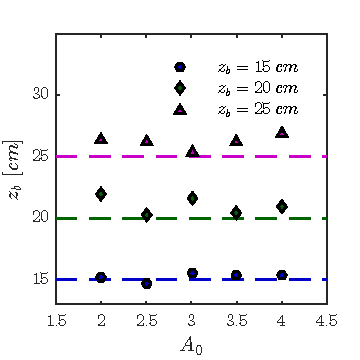
\includegraphics[height = 2.5in]{Figures/BreakHeight.pdf}}
\subfigure[]{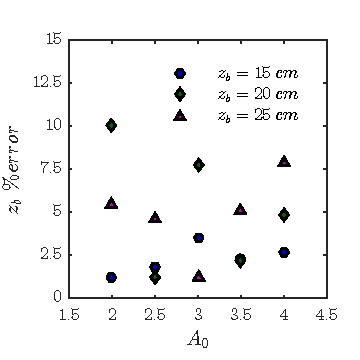
\includegraphics[height = 2.5in]{Figures/BreakHeightError.pdf}}
\caption{(a) Break height results for glycerin experiments as a function of expected break height and $A_b$, with the same fluid parameters as those in Fig.~\ref{fig:BreakEdge}. (b) Relative error in break height results.}
\label{fig:BreakHeightGlycerin}
\end{figure}

\begin{figure}
\centering
\subfigure[]{ 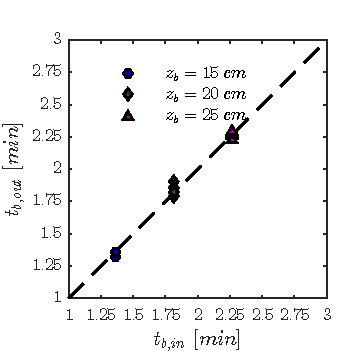
\includegraphics[height = 2.5in]{Figures/BreakTime.pdf}}
\subfigure[]{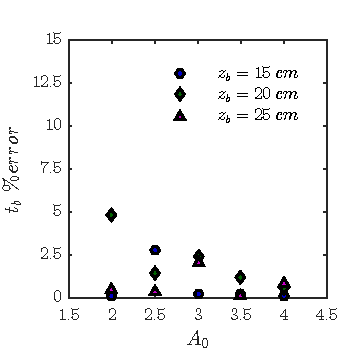
\includegraphics[height = 2.5in]{Figures/BreakTimeError.pdf}}
\caption{(a)Break time results for glycerin experiments compared to the expected break times, with the same fluid parameters as those in Fig.~\ref{fig:BreakEdge}. (b) Error in break height results.}
\label{fig:BreakTimeGlycerin}
\end{figure}  

\section{Discussion}\label{sec:Dis}
    Overall, we see high fidelity between the expected and observed breaking heights and times. The regions of large error in parameter space are likely due to a breakdown in our initial assumption that nonlinearity dominates over dispersion. For small $A_b$, nonlinearity does not have as large an effect as for other area ratios, and for large $z_b$, dispersion has more time to have a significant effect on the evolution of the boundary condition. \MM{Comparisons for $t_b$, numerics, dispersion/NL analysis, (corn syrup?)}

\section{Conclusion}\label{sec:Con}
    Using the dispersionless limit of a dispersive hydrodynamic system is an excellent approximation for non-oscillatory regions. By generating boundary conditions using this assumption, we are able to approximate a desired initial condition to $10\% $ accuracy. This method could be used for a variety of nonlinear dispersive systems for more accurate analysis of dispersive shock waves or other hydrodynamic structures that evolve from initial conditions.

\bibliography{bibfiles.bib}
\bibliographystyle{jfm}

\end{document}
%%% Local Variables: 
%%% mode: latex
%%% TeX-master: t
%%% End: 
